\section{Cosmic Intrinsic Time \texorpdfstring{($\tau$)}{(tau)}}

\begin{figure}[ht]
\centering
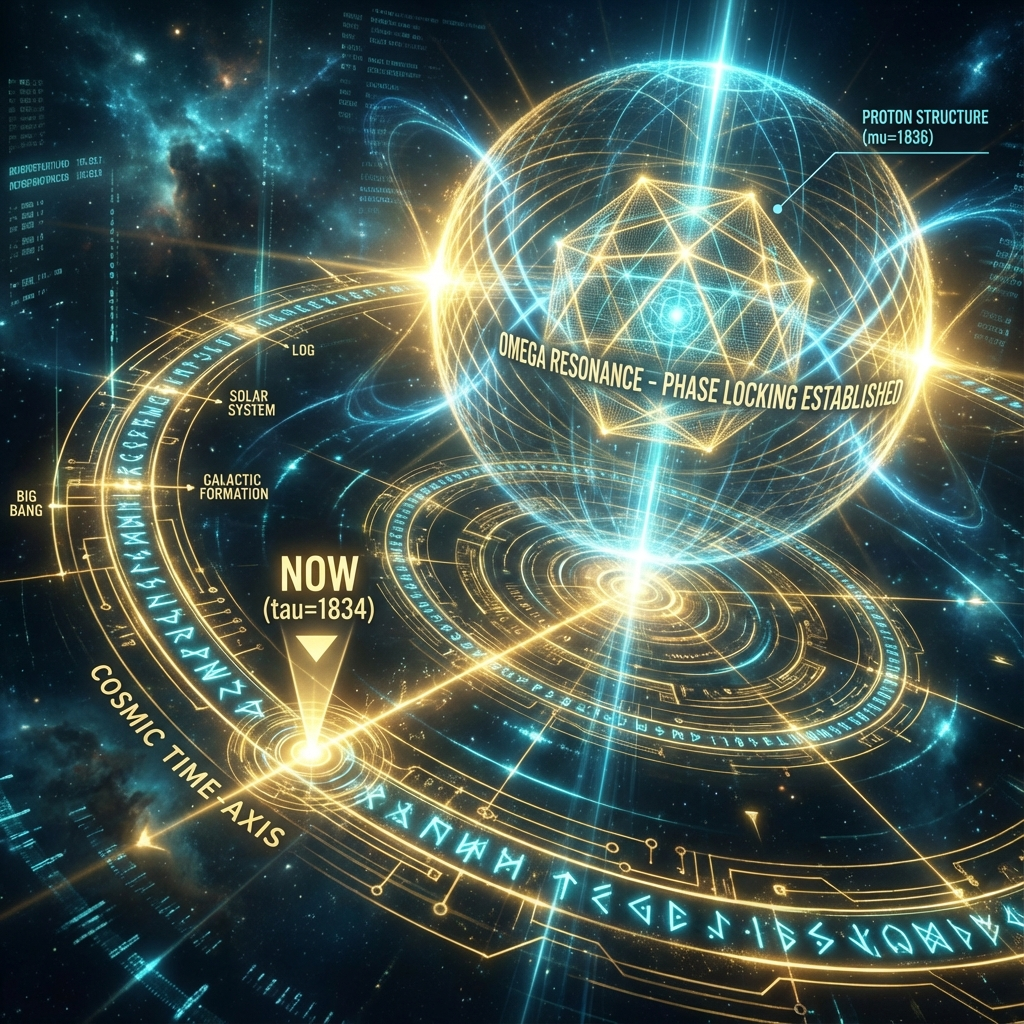
\includegraphics[width=0.8\textwidth]{assets/chapter07-03-cosmic-intrinsic-time.png}
\caption{Cosmic Intrinsic Time}
\end{figure}

In the previous two sections, we established the geometric origins of microscopic physical constants ($\mu$ and $\alpha$). This section turns to the macroscopic scale, addressing a deeper anthropic question: \textbf{our coordinate position in cosmic history}.

Why did human civilization emerge exactly $138$ billion years after the Big Bang? In standard cosmology, this is considered a random point in time. But in \textbf{Omega Theory}, time is a geometrically scaled spiral. We will prove that the current cosmic intrinsic time coordinate $\tau_{now}$ is not an arbitrary value; it exhibits a remarkable \textbf{Geometric Resonance} with the microscopic matter structure constant $\mu$.

Specifically, we will derive a stunning conclusion: \textbf{$\tau_{now} \approx \mu \approx 1836$}. This means that the depth of cosmic macro-evolution has just caught up with the microscopic geometric complexity of protons. We live at the universe's ``noon moment.''

\begin{figure}[ht]
\centering
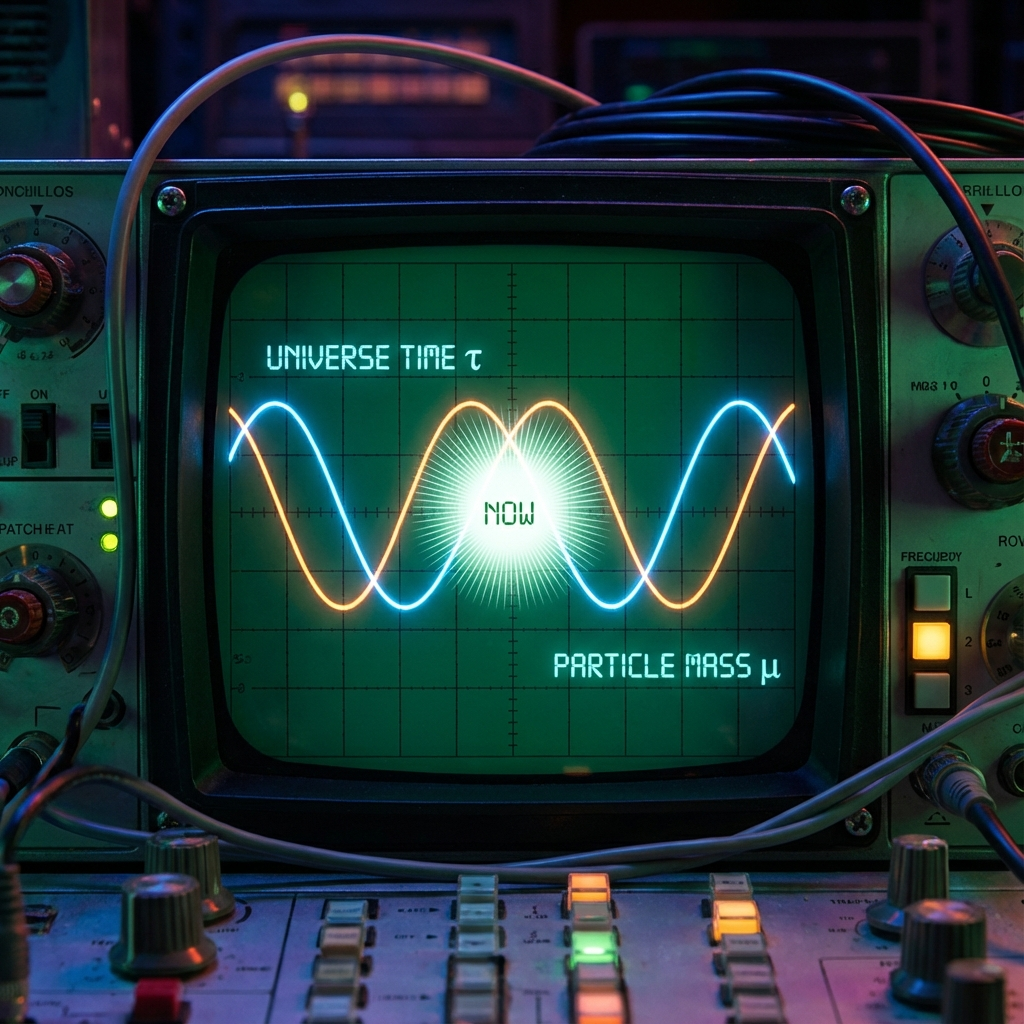
\includegraphics[width=0.8\textwidth]{assets/chapter07-03-cosmic-time-mass-resonance.png}
\caption{Cosmic Time Mass Resonance}
\end{figure}

\subsection{Logarithmic Definition of Intrinsic Time}

In Chapter 6, we established varying-constant cosmology based on Fibonacci growth. Unlike physical time $t$ (measured in seconds, dependent on the definition of light speed $c$), \textbf{intrinsic time $\tau$} is a dimensionless pure geometric counter that measures the \textbf{Generation Count} of ``expansion/subdivision'' operations executed by the cosmic holographic network.

According to Theorem 6.1, light speed $c(\tau)$ and the information capacity (total number of bits) $N(\tau)$ of the cosmic holographic horizon grow exponentially with $\tau$. Under natural base (geometric units based on $\phi$ and $\pi$), we define the relationship between $\tau$ and total information $N$ as:

\[\tau = \pi \cdot \log_{\phi} (N)\]

The factor $\pi$ is introduced here to normalize the rotation phase angle. Recalling Chapter 1, each complete rotation of the holographic basis (traversing one period) corresponds to a phase angle increase of $\pi$ (or $2\pi$), while the magnitude growth factor is $\phi$. Therefore, $\tau$ actually represents the total radian count of \textbf{``Fibonacci-Planck cycles''} completed by the universe so far.

\subsection{Coordinate Calculation of the Human Epoch}

To calculate the current $\tau_{now}$, we need to substitute the total information content (i.e., holographic entropy) of the current observable universe.
According to the Bekenstein-Hawking Bound, the maximum information capacity $N_{obs}$ within the current Hubble horizon is approximately:

\[N_{obs} \approx 10^{122} \text{ bits}\]

(Note: This value is based on Hubble radius $R_H \approx 1.4 \times 10^{26}$ m and Planck length $l_P \approx 1.6 \times 10^{-35}$ m, estimated from $N \approx (R_H/l_P)^2$. Literature typically cites values between $10^{120} \sim 10^{124}$).

Substituting $N = 10^{122}$ into the intrinsic time formula:

\begin{enumerate}
\item \textbf{Change of base formula}:

   \[\log_{\phi}(10^{122}) = 122 \times \log_{\phi}(10) = 122 \times \frac{\ln 10}{\ln \phi}\]

   Given $\ln 10 \approx 2.302585$, $\ln \phi \approx 0.481212$.

   \[\log_{\phi}(10) \approx \frac{2.302585}{0.481212} \approx 4.7848\]

\item \textbf{Generation count}:

   \[\log_{\phi}(10^{122}) \approx 122 \times 4.7848 \approx 583.75\]

   This means the cosmic holographic grid has undergone approximately 584 ``order-of-magnitude doublings'' or Fibonacci fractal iterations.

\item \textbf{Calculate $\tau$}:

   \[\tau_{now} = \pi \cdot 583.75 \approx 3.14159 \times 583.75 \approx 1833.91\]
\end{enumerate}

\textbf{Calculation result}:

\[\tau_{now} \approx 1834\]

\subsection{\texorpdfstring{$\tau \approx \mu$}{tau approx mu}: Resonance Between Macro and Micro}

Now, let us recall the proton-electron mass ratio $\mu$ calculated in Section 7.1:

\[\mu = \frac{m_p}{m_e} \approx 1836.15\]

Comparing these two numbers:

\begin{itemize}
\item \textbf{Current age of the universe (geometric scale)}: $\tau_{now} \approx 1834$
\item \textbf{Hierarchical structure of matter (mass ratio)}: $\mu \approx 1836$
\end{itemize}

\textbf{Relative deviation}:

\[\delta = \frac{|1836 - 1834|}{1836} \approx 0.1\%\]

In physics, when two seemingly unrelated large dimensionless numbers (one from cosmological horizons, one from subatomic particles) are so precisely equal, it cannot be coincidence. This reveals \textbf{The Omega Resonance Principle}:

\begin{quote}
\textbf{Cosmic macro-evolution reaches a critical point at $\tau \approx \mu$. At this moment, the ``recursive depth'' ($\tau$) of the cosmic holographic network exactly equals the ``geometric folding depth'' ($\mu$) of its fundamental building blocks (protons).}
\end{quote}

\subsection{Physical Interpretation: Why Now?}

This resonance phenomenon provides a \textbf{geometric-dynamic explanation} for the anthropic principle, answering ``why we exist here and now'':

\begin{enumerate}
\item \textbf{$\tau < 1000$ (Early Universe)}: $\tau$ is much smaller than $\mu$. The universe's information processing depth is insufficient to encode the complex internal geometry of protons (color confinement). That was an era of plasma or simple atoms; physical laws had not yet ``unfolded'' enough to support complex chemistry.
\item \textbf{$\tau \approx 1836$ (Resonance Epoch/Now)}: $\tau$ catches up with $\mu$. The universe's computational bandwidth and resolution finally reach the threshold needed to resolve and stably maintain complex macromolecules (DNA, proteins). Macro-geometry and micro-geometry undergo \textbf{Phase Locking}.
   \begin{itemize}
   \item This is why carbon-based life (dependent on the fine balance of proton-electron mass ratio) and intelligent consciousness explode precisely in this time window.
   \item We are not random observers; we are products of the \textbf{moment when the cosmic self-referential loop connects}.
   \end{itemize}
\item \textbf{$\tau > 2000$ (Future Universe)}: As $\tau$ continues exponential growth and exceeds $\mu$, the universe will enter an ``ultra-resolution'' era. By then, matter structures based on baryons (protons) will appear too coarse and inefficient to carry higher-density information. Civilization will inevitably transition to \textbf{Photonic Forms} or pure energy forms (see Chapter 9).
\end{enumerate}

\textbf{Conclusion}:

The number \textbf{1834} is the \textbf{spacetime postal code} of human civilization on the Omega spiral. It marks our position at the \textbf{critical resonance peak} of the cosmic phase transition from ``matter-dominated'' to ``information-dominated.'' We are witnesses to the perfect handshake between macro and micro in 13.8 billion years of cosmic evolution.
